% Provenance (never printed): cycle 4 SVT, "La planete Terre, l'environnement
% et l'action humaine": resources from the Earth, their geological origin, the
% time they take to form and the rate we use them; see
% sources/book1/PROVENANCE.md. Book 1, grade 9, chapter 3.
% Vocabulary guard: owns ore deposit (with concentration factor), aggregate,
% reserve. Resource, renewable resource, ore, raw material (chemistry grade
% 5), fossil fuels (chemistry grade 8) and element abundances (chemistry
% grade 9) are recalled in prose. Groundwater and aquifers are g6's. Coal,
% oil and gas are told, not defined: "source rock", "reservoir", "seal",
% "trap" and the coal ranks belong to Book 2 g11 (fossil-fuel-geology);
% "hydrothermal" is not used (later books). Scientific notation (grade 9).
\chapter{Resources from the Earth}\label{ch:g9:earth-resources}

A smartphone fits in a pocket, yet it holds dozens of chemical elements:
copper for its wires, neodymium for the magnets of its speaker, gallium
for the light of its screen, indium for the thin coating of its screen
that carries electricity, and many more. Every one of them was dug out of the ground
somewhere on the Earth. A house holds far more: an average family house
needs about a hundred tonnes of \omterm{def:g3:stones-pebbles-sand:sand}{sand}, \omterm{def:g3:stones-pebbles-sand:pebble}{gravel} and crushed stone, and its
share of the streets and schools around it about three times as much.
Where in the Earth are these materials found, and why there?
% ledger: usgs:smartphone, usgs:aggregate (114 and 328 short tons: about 100 and 300 t)

\begin{recall}
In chemistry, you learn that the materials we take from nature are
\emph{resources}; an \emph{ore} is a \omterm{def:g3:stones-pebbles-sand:rock}{rock} from which a metal can be
extracted; a \emph{renewable} resource is renewed by nature as fast as we
use it; coal, oil and natural gas are \emph{\omterm{def:g7:sediments-and-fossils:fossil}{fossil} fuels}; and oxygen,
silicon, aluminium and iron are the most abundant elements of the \omterm{def:g6:inside-the-earth:layers}{crust}.
\omterm{def:g6:water-underground:groundwater}{Groundwater} fills the \omterm{def:g6:water-underground:porosity}{pores} of an \omterm{def:g6:water-underground:aquifer}{aquifer}, and \omterm{def:g4:clouds-rain-snow:precipitation}{rain} refills it
(\cref{ch:g6:water-underground}). \omterm{def:g7:sediments-and-fossils:sediment}{Sediments} pile up in layers and become
\omterm{def:g6:rocks-and-minerals:rock-families}{sedimentary rocks} (\cref{ch:g7:sediments-and-fossils}), over times counted
in millions of years (\cref{ch:g7:geological-time}).
\end{recall}

\section{Why a metal has to be concentrated}

Copper is everywhere: an ordinary \omterm{def:g3:stones-pebbles-sand:rock}{rock} holds a little of it, a few grams in
every hundred kilograms. But to get one kilogram of copper out of such a
\omterm{def:g3:stones-pebbles-sand:rock}{rock}, you would have to dig, crush and treat tonnes of it. Mining is worth
the cost only where nature has gathered the metal into a much richer \omterm{def:g3:stones-pebbles-sand:rock}{rock}.
% ledger: perkins:ore-grades (copper 0.006 % of the crust)

\begin{definition}[Ore deposit and concentration factor]\label{def:g9:earth-resources:ore-deposit}
An \emph{ore deposit}\index{ore deposit} is a body of \omterm{def:g3:stones-pebbles-sand:rock}{rock} in which
natural processes have concentrated a metal or a \omterm{def:g6:rocks-and-minerals:mineral}{mineral} enough for it to
be extracted at a profit. The \emph{concentration
factor}\index{concentration factor} of a metal is the number of times its
content in the ore is greater than its average content in the \omterm{def:g6:inside-the-earth:layers}{crust}:
\[
\text{concentration factor} = \frac{\text{content in the ore}}{\text{average content in the crust}} .
\]
\end{definition}
% ledger: perkins:ore-grades, earle:ore-grades

The common metals of the \omterm{def:g6:inside-the-earth:layers}{crust}, aluminium and iron, need to be concentrated
only about four times. Copper needs about 80 times, zinc about 600 times,
and the rarest metals of the chart, gold, tin and chromium, thousands of
times. The rarer a metal in the \omterm{def:g6:inside-the-earth:layers}{crust}, the more nature has to work to make
an ore of it, and the fewer places where it has done so.
% ledger: perkins:ore-grades, earle:ore-grades

\begin{example}[Copper]
The \omterm{def:g6:inside-the-earth:layers}{crust} holds on average \qty{0.006}{\%} of copper; a copper ore can be
mined from about \qty{0.5}{\%}. The \omterm{def:g9:earth-resources:ore-deposit}{concentration factor} is $0.5 \div 0.006
\approx 83$, about 80, or close to $10^2$. Another textbook takes \qty{40}{ppm}
(\qty{0.004}{\%}) for ordinary \omterm{def:g3:stones-pebbles-sand:rock}{rock} and \qty{1}{\%} for the ore: $1 \div
0.004 = 250$. The two numbers differ, but both say the same thing: a
copper ore is about a hundred times richer than ordinary \omterm{def:g3:stones-pebbles-sand:rock}{rock}.
\end{example}
% ledger: perkins:ore-grades, earle:ore-grades

\begin{omfigure}
\begin{tikzpicture}
\begin{axis}[xbar, xmode=log, width=12cm, height=5.3cm, xmin=1, xmax=2e4,
  log origin=infty, bar width=9pt, enlarge y limits=0.1,
  ytick=data, yticklabels from table={figdata/out/grade-9-concentration.dat}{metal},
  y dir=reverse, xlabel={concentration factor (logarithmic scale)},
  xtick={1,10,100,1000,10000}, xticklabels={$1$,$10$,$10^2$,$10^3$,$10^4$},
  tick label style={font=\footnotesize}, label style={font=\small},
  nodes near coords, nodes near coords style={font=\scriptsize, anchor=west},
  point meta=explicit, xmajorgrids, grid style={black!12}]
\addplot[fill=omWarm!45, draw=omWarm!80!black] table[x=factor, y=x, meta=factor] {figdata/out/grade-9-concentration.dat};
\end{axis}
\end{tikzpicture}

{\small How many times nature has to concentrate seven metals to make an
ore worth mining: the minimum grade of the ore divided by the average
content of the \omterm{def:g6:inside-the-earth:layers}{crust}. Each step of the scale is ten times the one before.
Data: D.~Perkins and others, \emph{Mineralogy}, and, for gold,
S.~Earle, \emph{Environmental Geology}.}
% ledger: perkins:ore-grades, earle:ore-grades (figdata/grade-9/concentration.py)
\label{fig:g9:earth-resources:factors}
\end{omfigure}

\begin{method}[Computing a concentration factor]
\begin{enumerate}
  \item Write the content of the metal in the ore and in the average \omterm{def:g6:inside-the-earth:layers}{crust}
        in the same unit (percent, or grams per tonne).
  \item Divide the content in the ore by the content in the \omterm{def:g6:inside-the-earth:layers}{crust}.
  \item Round the result: what matters is its size, about 10, 100 or
        1000, which you can write as a power of ten.
\end{enumerate}
\end{method}


\section{How ore deposits form}

Nature concentrates metals in several ways. Three of them are shown below.

\begin{omfigure}
\begin{tikzpicture}[x=1cm, y=1cm, font=\footnotesize, >={Stealth[length=2mm]}]
  % country rock
  \fill[black!13] (0,0) rectangle (13,4.6);
  % surface with a valley on the right
  \fill[white] (0,4.6) -- (8.4,4.6) -- (9.6,3.7) -- (11.2,3.7) -- (12.0,4.6) -- (13,4.6) -- (13,5.6) -- (0,5.6) -- cycle;
  \draw[black!60] (0,4.6) -- (8.4,4.6) -- (9.6,3.7) -- (11.2,3.7) -- (12.0,4.6) -- (13,4.6);
  % river gravels on the valley floor
  \fill[omLithCongl] (9.5,3.75) -- (11.3,3.75) -- (11.15,3.35) -- (9.65,3.35) -- cycle;
  \foreach \x in {9.8,10.1,10.45,10.8,11.05} \fill[black!45] (\x,3.6) circle (0.05);
  \foreach \x in {9.9,10.3,10.65,10.95} \fill[yellow!80!orange] (\x,3.4) circle (0.045);
  \fill[omRiver!60] (9.9,3.75) rectangle (10.9,3.85);
  % magma body (cooling granite)
  \fill[omLithGranite] (1.0,0) .. controls (1.2,1.6) and (2.2,2.1) .. (3.4,2.1)
     .. controls (4.6,2.1) and (5.6,1.6) .. (5.8,0) -- cycle;
  \draw[black!50] (1.0,0) .. controls (1.2,1.6) and (2.2,2.1) .. (3.4,2.1)
     .. controls (4.6,2.1) and (5.6,1.6) .. (5.8,0);
  % heavy minerals settled at the bottom of the magma body
  \fill[black!60] (1.05,0) rectangle (5.75,0.25);
  % cracks and veins above the magma
  \foreach \x/\a in {2.6/12, 3.4/-6, 4.3/-15} {
    \draw[black, line width=1.6pt] (\x,2.15) -- ++(90+\a:2.0);
    \draw[yellow!80!orange, line width=0.6pt] (\x,2.15) -- ++(90+\a:2.0);
  }
  % hot water rising
  \draw[->, omWarm, thick] (2.1,1.9) .. controls (1.9,2.7) and (2.2,3.2) .. (2.45,3.7);
  \draw[->, omWarm, thick] (4.95,1.7) .. controls (5.1,2.6) and (4.8,3.3) .. (4.55,3.8);
  % labels
  \node[anchor=north, align=center] at (3.4,1.35) {a cooling body of magma};
  \node[anchor=west, align=left, fill=white, fill opacity=0.85, text opacity=1, inner sep=1.5pt] at (6.2,0.75)
    {\textbf{1} heavy metal-rich minerals\\ settle at the bottom};
  \draw[black!70] (6.15,0.65) -- (5.5,0.15);
  \node[anchor=west, align=left, fill=white, fill opacity=0.85, text opacity=1, inner sep=1.5pt] at (5.6,2.55)
    {\textbf{2} hot water rises through cracks,\\ cools and leaves metals: veins};
  \draw[black!70] (5.55,2.6) -- (4.2,3.3);
  \node[anchor=south, align=center] at (10.4,4.7) {\textbf{3} grains of gold settle with\\ the gravel of a river: a placer};
  \draw[black!70] (10.4,4.7) -- (10.3,3.45);
  \node[anchor=south west] at (0.1,4.65) {ground surface};
\end{tikzpicture}

{\small Three ways to concentrate a metal (a sketch, not to scale). (1) In
a body of \omterm{def:g7:volcanoes:magma}{magma}, heavy \omterm{def:g6:rocks-and-minerals:mineral}{minerals} rich in nickel or copper sink and gather at
the bottom. (2) \omterm{def:g6:water-underground:groundwater}{Groundwater} heated by the \omterm{def:g7:volcanoes:magma}{magma}, and water given off by the
\omterm{def:g7:volcanoes:magma}{magma} itself, dissolve metals, rise through cracks and drop them where the
\omterm{def:g3:stones-pebbles-sand:rock}{rock} is cooler, filling the cracks with veins. (3) \omterm{def:g5:water-shapes-the-land:erosion}{Erosion} frees gold from
the veins; the \omterm{def:g1:landscapes-around-us:water}{river} carries it, and the heavy grains settle among the
\omterm{def:g3:stones-pebbles-sand:pebble}{gravels}, down to the \omterm{def:g3:stones-pebbles-sand:rock}{bedrock}.}
% ledger: earle:magmatic, usgs:gold-lode, usgs:gold-placer
\label{fig:g9:earth-resources:deposits}
\end{omfigure}

\paragraph{In the magma.} When a body of \omterm{def:g7:volcanoes:magma}{magma} cools, the \omterm{def:g6:rocks-and-minerals:mineral}{minerals} that
crystallize first are not always the lightest. In \omterm{def:g7:volcanoes:magma}{magmas} from the \omterm{def:g6:inside-the-earth:layers}{mantle},
heavy \omterm{def:g6:rocks-and-minerals:mineral}{minerals} rich in nickel and copper sink to the bottom and gather into
a rich layer. Most of the nickel mined in the world comes from deposits of
this kind.
% ledger: earle:magmatic

\paragraph{In cracks, from hot water.} \omterm{def:g6:water-underground:groundwater}{Groundwater} that flows near a body
of \omterm{def:g7:volcanoes:magma}{magma}, a few kilometres below the surface, is heated and rises through
the cracks of the \omterm{def:g3:stones-pebbles-sand:rock}{rock}. Hot water dissolves metals from the \omterm{def:g3:stones-pebbles-sand:rock}{rocks} it
crosses. When it reaches cooler \omterm{def:g3:stones-pebbles-sand:rock}{rock} nearer the surface, the metals come
out of the water as \omterm{def:g6:rocks-and-minerals:mineral}{minerals} and fill the cracks: these are
\emph{veins}\index{vein}. Many gold deposits are veins of this kind. Around
some bodies of \omterm{def:g7:volcanoes:magma}{magma}, hot water has crossed a whole mass of broken \omterm{def:g3:stones-pebbles-sand:rock}{rock}
and left copper in it, spread out but over a huge volume: these are the
largest copper deposits in the world.
% ledger: usgs:gold-lode, earle:porphyry

\begin{omfigure}
\begin{minipage}[c]{0.46\linewidth}\centering
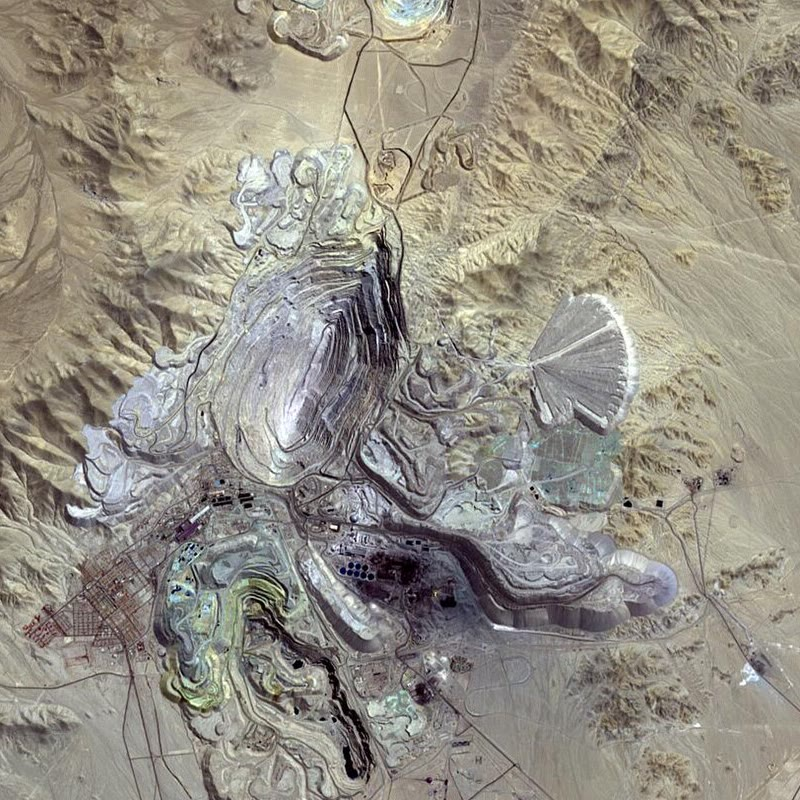
\includegraphics[width=\linewidth]{images/book1/g9-chuquicamata.jpg}
\end{minipage}\hfill
\begin{minipage}[c]{0.5\linewidth}\raggedright
{\small The Chuquicamata copper mine, in the Atacama \omterm{def:g5:weather-and-climate:desert}{Desert} of Chile, seen
by the ASTER instrument on a NASA satellite in 2007 (the image is about
\qty{12}{km} across). The oval pit in the middle, worked for over a
century, is \qty{4.3}{km} long, \qty{2.7}{km} wide and \qty{1.1}{km}
deep. NASA/METI/AIST/Japan
Space Systems and the U.S./Japan ASTER Science Team (public domain, via
Wikimedia Commons).}
\end{minipage}
% ledger: commons:chuquicamata, earle:chuquicamata
\label{fig:g9:earth-resources:chuquicamata}
\end{omfigure}

\paragraph{In river gravels.} Gold does not rust and hardly weathers. When
\omterm{def:g5:water-shapes-the-land:erosion}{erosion} wears down a gold vein, the gold is freed as dust, flakes, grains
and sometimes nuggets, and \omterm{def:g1:landscapes-around-us:water}{rivers} carry it downstream. Gold is very dense:
about \qty{19}{g/cm^3} pure, against about \qty{2.5}{g/cm^3} for ordinary
\omterm{def:g3:stones-pebbles-sand:rock}{rock}. In \omterm{def:g5:water-shapes-the-land:flood}{floods}, when the whole bed of \omterm{def:g3:stones-pebbles-sand:sand}{sand} and \omterm{def:g3:stones-pebbles-sand:pebble}{gravel} moves, the heavy
grains of gold work their way down and collect on the \omterm{def:g3:stones-pebbles-sand:rock}{bedrock}. Geologists
call such deposits \emph{placers}\index{placer}.
% ledger: usgs:gold-placer

\section{Coal, oil and gas}

Coal, oil and natural gas are the remains of living things, buried before
they could rot. Almost all the organic matter of a dead plant or animal is
turned back into carbon dioxide within weeks to decades. Only the part cut
off from the oxygen of the air, at the bottom of a stagnant swamp or of a
deep \omterm{def:g2:water-on-earth:ocean}{sea}, can be buried and kept for millions of years.
% ledger: earle:coal, earle:oil-gas

\begin{omfigure}
\begin{minipage}[c]{0.46\linewidth}\centering
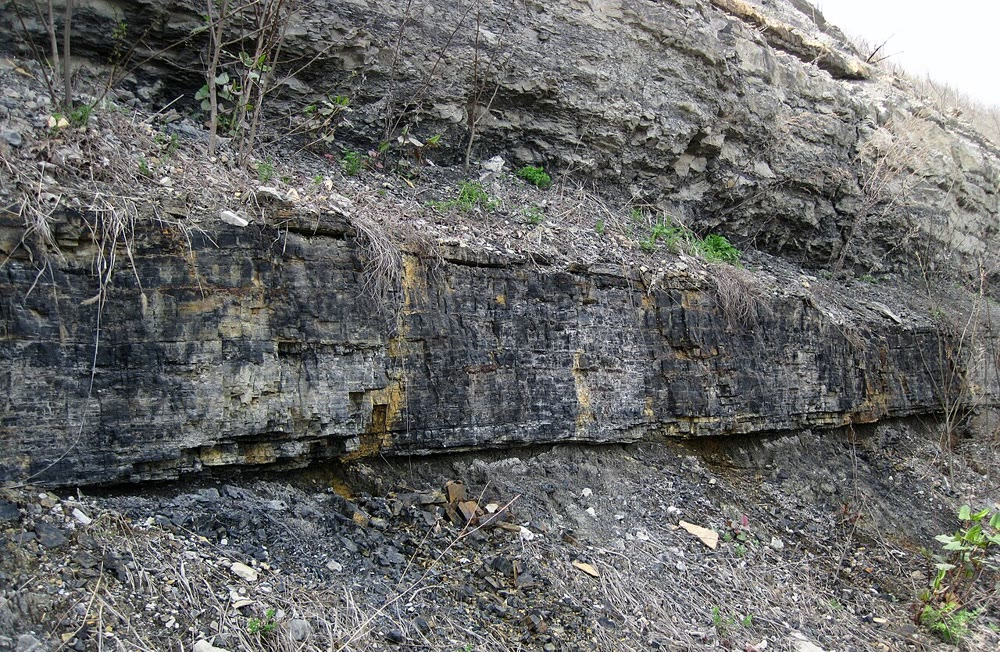
\includegraphics[width=\linewidth]{images/book1/g9-coal-seam.jpg}
\end{minipage}\hfill
\begin{minipage}[c]{0.5\linewidth}\raggedright
{\small A seam of coal, the dark layer across the middle, between
\omterm{def:g6:rocks-and-minerals:rock-families}{sedimentary rocks}, beside a road in Ohio, United States. The seam lies flat,
as the swamp did. Photograph by James St.~John (CC BY 2.0, via Wikimedia
Commons).}
\end{minipage}
% ledger: commons:meigs-coal
\label{fig:g9:earth-resources:coal-seam}
\end{omfigure}


\paragraph{Coal.} Coal starts in swamps beside \omterm{def:g1:landscapes-around-us:water}{rivers} and \omterm{def:g5:water-shapes-the-land:delta}{deltas}, in warm
and wet \omterm{def:g5:weather-and-climate:climate}{climates}, where plants grow fast. Dead trunks and leaves fall into
still water that holds little oxygen, and do not rot. The swamp has to last
for centuries to millennia to build a thick layer. One day a \omterm{def:g1:landscapes-around-us:water}{river} changes
course or \omterm{def:g5:water-shapes-the-land:flood}{floods}, and covers the swamp with \omterm{def:g3:stones-pebbles-sand:sand}{sand} and \omterm{def:g3:stones-pebbles-sand:sand}{mud}. As more
\omterm{def:g7:sediments-and-fossils:sediment}{sediments} pile up, the plant layer is pressed and heated, and turns into
coal: first a soft, brown coal with about a third of carbon, some hundreds
of metres down; a hard black coal, with up to 86~\% of carbon, a few
kilometres down. The coal mined today in the United States, for instance,
is mostly 100 to 300~million years old.
% ledger: earle:coal, eia:coal

\begin{omfigure}
\begin{tikzpicture}[x=1cm, y=0.8cm, font=\footnotesize]
  \foreach \i/\t in {0/{(a) a swamp forest:\\ dead plants pile up\\ under still water},
                     1/{(b) buried under river\\ sand and mud, the\\ layer is squeezed},
                     2/{(c) deeper and warmer\\ (hundreds of metres):\\ soft brown coal},
                     3/{(d) deeper still\\ (kilometres):\\ hard black coal}} {
    \begin{scope}[xshift=\i*3.35cm]
      \draw[black!40] (0,0) rectangle (2.9,4.2);
      \node[align=center, anchor=north, font=\scriptsize] at (1.45,-0.1) {\t};
    \end{scope}
  }
  % (a) swamp: water, trees, plant layer
  \fill[omSea] (0,2.6) rectangle (2.9,3.1);
  \fill[brown!60!black!70] (0,2.0) rectangle (2.9,2.6);
  \fill[omLithShale] (0,0) rectangle (2.9,2.0);
  \foreach \x in {0.5,1.4,2.3} {
    \draw[brown!50!black, line width=1.2pt] (\x,2.6) -- (\x,3.7);
    \fill[green!45!black] (\x,3.85) circle (0.3);
  }
  % (b) buried
  \begin{scope}[xshift=3.35cm]
    \fill[lith sandstone] (0,2.6) rectangle (2.9,4.0);
    \fill[brown!55!black!80] (0,2.2) rectangle (2.9,2.6);
    \fill[omLithShale] (0,0) rectangle (2.9,2.2);
    \draw[->, thick] (1.45,4.15) -- (1.45,3.45);
  \end{scope}
  % (c) lignite
  \begin{scope}[xshift=6.7cm]
    \fill[lith sandstone] (0,1.9) rectangle (2.9,4.2);
    \fill[brown!45!black] (0,1.65) rectangle (2.9,1.9);
    \fill[omLithShale] (0,0) rectangle (2.9,1.65);
  \end{scope}
  % (d) coal
  \begin{scope}[xshift=10.05cm]
    \fill[lith sandstone] (0,1.25) rectangle (2.9,4.2);
    \fill[black!85] (0,1.1) rectangle (2.9,1.25);
    \fill[omLithShale] (0,0) rectangle (2.9,1.1);
  \end{scope}
\end{tikzpicture}

{\small From a swamp to a coal seam (a sketch, not to scale). As the layer
of plants sinks deeper, it is pressed and heated: water and gases leave it,
it gets thinner, and its share of carbon rises.}
% ledger: earle:coal, eia:coal
\label{fig:g9:earth-resources:coal}
\end{omfigure}


\paragraph{Oil and gas.} Oil and most natural gas come from the tiny
plants and animals that live in the \omterm{def:g2:water-on-earth:ocean}{sea}, such as diatoms. Their remains
sink with the \omterm{def:g3:stones-pebbles-sand:sand}{mud} to the \omterm{def:g2:water-on-earth:ocean}{sea} floor, and some are buried before they decay.
Millions of years and kilometres of \omterm{def:g7:sediments-and-fossils:sediment}{sediment} later, heat and pressure
change them: below about \qty{2}{km}, between about 60 and
\qty{120}{\degreeCelsius}, into oil; hotter still, into gas. Oil and gas
are lighter than water. They creep slowly upwards through the \omterm{def:g6:water-underground:porosity}{pores} of
\omterm{def:g6:water-underground:permeability}{permeable} \omterm{def:g3:stones-pebbles-sand:rock}{rocks}, and many reach the surface and are lost. The ones we find
were stopped on their way by a layer of \omterm{def:g6:water-underground:permeability}{impermeable} \omterm{def:g3:stones-pebbles-sand:rock}{rock}, often at the
top of an upfold, where they gather: gas at the top, oil below it, and
water underneath.
% ledger: eia:oil, eia:gas, earle:oil-gas

\begin{omfigure}
\begin{tikzpicture}[x=1cm, y=1cm, font=\footnotesize, >={Stealth[length=2mm]}]
  \def\fold#1{(0,#1) .. controls (3,#1+1.0) and (4.0,#1+1.6) .. (6,#1+1.6) .. controls (8.0,#1+1.6) and (9,#1+1.0) .. (12,#1)}
  % layers from the bottom up
  \fill[omLithShale!60!black!40] (0,0) -- \fold{0.9} -- (12,0) -- cycle;
  \fill[lith sandstone] \fold{0.9} -- (12,2.1) -- (12,2.1) .. controls (9,3.1) and (8.0,3.7) .. (6,3.7) .. controls (4.0,3.7) and (3,3.1) .. (0,2.1) -- cycle;
  \fill[lith shale] (0,2.1) .. controls (3,3.1) and (4.0,3.7) .. (6,3.7) .. controls (8.0,3.7) and (9,3.1) .. (12,2.1) -- (12,3.6) .. controls (9,4.6) and (8.0,5.2) .. (6,5.2) .. controls (4.0,5.2) and (3,4.6) .. (0,3.6) -- cycle;
  \fill[lith sandstone] (0,3.6) .. controls (3,4.6) and (4.0,5.2) .. (6,5.2) .. controls (8.0,5.2) and (9,4.6) .. (12,3.6) -- (12,5.6) -- (0,5.6) -- cycle;
  % gas and oil under the crest of the impermeable layer
  \fill[omWxSun!60] (4.55,3.55) .. controls (5.2,3.69) and (6.8,3.69) .. (7.45,3.55) -- (7.1,3.35) -- (4.9,3.35) -- cycle;
  \fill[black!75] (4.9,3.35) -- (7.1,3.35) -- (8.05,3.05) .. controls (7.0,3.15) and (5.0,3.15) .. (3.95,3.05) -- cycle;
  % arrows: oil creeping up through the permeable layer
  \draw[->, black, thick] (1.4,2.05) -- (2.4,2.55);
  \draw[->, black, thick] (10.6,2.05) -- (9.6,2.55);
  \draw[->, black!70] (3.0,2.65) -- (3.8,2.95);
  \draw[->, black!70] (9.0,2.65) -- (8.2,2.95);
  % labels
  \node[anchor=west, fill=white, fill opacity=0.85, text opacity=1, inner sep=1.5pt] at (0.1,0.45) {dark mud of the old sea floor: oil and gas form here};
  \node[anchor=east, fill=white, fill opacity=0.85, text opacity=1, inner sep=1.5pt] at (11.9,1.9) {permeable sandstone};
  \node[anchor=east, fill=white, fill opacity=0.85, text opacity=1, inner sep=1.5pt] at (11.9,3.25) {impermeable shale};
  \node[anchor=south, fill=white, fill opacity=0.85, text opacity=1, inner sep=1.5pt] at (6,5.25) {surface rocks};
  \node[font=\scriptsize] at (6,3.48) {gas};
  \node[font=\scriptsize, text=white] at (6,3.22) {oil};
\end{tikzpicture}

{\small Oil and gas stopped under an \omterm{def:g6:water-underground:permeability}{impermeable} layer at the top of an
upfold (a sketch, not to scale; the water that fills the rest of the
sandstone is not shown). Below the fold, they creep up through the
\omterm{def:g6:water-underground:permeability}{permeable} sandstone (arrows) and gather under the crest: gas on top, oil
below.}
% ledger: earle:oil-gas
\label{fig:g9:earth-resources:oil}
\end{omfigure}

\section{Water from the ground}

\omterm{def:g6:water-underground:groundwater}{Groundwater} is also a resource from the Earth, the one we use every day.
Unlike a metal or coal, it is renewed: \omterm{def:g4:clouds-rain-snow:precipitation}{rain} refills the \omterm{def:g6:water-underground:aquifer}{aquifers}. But it
is renewed slowly, and only as fast as \omterm{def:g4:clouds-rain-snow:precipitation}{rain} soaks in. An \omterm{def:g6:water-underground:aquifer}{aquifer} pumped
faster than it is refilled sees its \omterm{def:g6:water-underground:water-table}{water table} fall, and \omterm{def:g6:water-underground:spring}{wells} run dry
(\cref{ch:g6:water-underground}). \omterm{def:g6:water-underground:groundwater}{Groundwater} is a renewable resource
only as long as it is not drawn faster than it is renewed.
% ledger: wss:aquifer

\section{Sand and gravel}

The solid material that people dig out of the ground in the largest amounts
is neither coal nor a metal ore: it is \omterm{def:g3:stones-pebbles-sand:sand}{sand} and \omterm{def:g3:stones-pebbles-sand:pebble}{gravel}.
% ledger: tos:sand

\begin{definition}[Aggregate]\label{def:g9:earth-resources:aggregate}
\emph{Aggregates}\index{aggregate} are the \omterm{def:g3:stones-pebbles-sand:sand}{sand}, the \omterm{def:g3:stones-pebbles-sand:pebble}{gravel} and the
crushed stone used in building: in concrete, under roads and railways,
and to fill the ground.
\end{definition}
% ledger: usgs:aggregate, tos:sand

Most \omterm{def:g3:stones-pebbles-sand:sand}{sand} goes into concrete, a mix of \omterm{def:g3:stones-pebbles-sand:sand}{sand}, \omterm{def:g3:stones-pebbles-sand:pebble}{gravel}, water and cement. In
2019 the world needed about 50~billion tonnes of \omterm{def:g3:stones-pebbles-sand:sand}{sand} and \omterm{def:g3:stones-pebbles-sand:pebble}{gravel} a year,
that is $5 \times 10^{10}$ tonnes, or about \qty{18}{kg} for every person
on the Earth, every day. \omterm{def:g3:stones-pebbles-sand:sand}{Sand} and \omterm{def:g3:stones-pebbles-sand:pebble}{gravel} are dug from pits on land, from
riverbeds and, more and more, from the \omterm{def:g2:water-on-earth:ocean}{sea} floor. Taken from a \omterm{def:g1:landscapes-around-us:water}{river}, they
leave less \omterm{def:g3:stones-pebbles-sand:sand}{sand} to reach the \omterm{def:g1:landscapes-around-us:water}{coast}, and beaches downstream wear away.
% ledger: tos:sand

\begin{omfigure}
\begin{minipage}[c]{0.46\linewidth}\centering
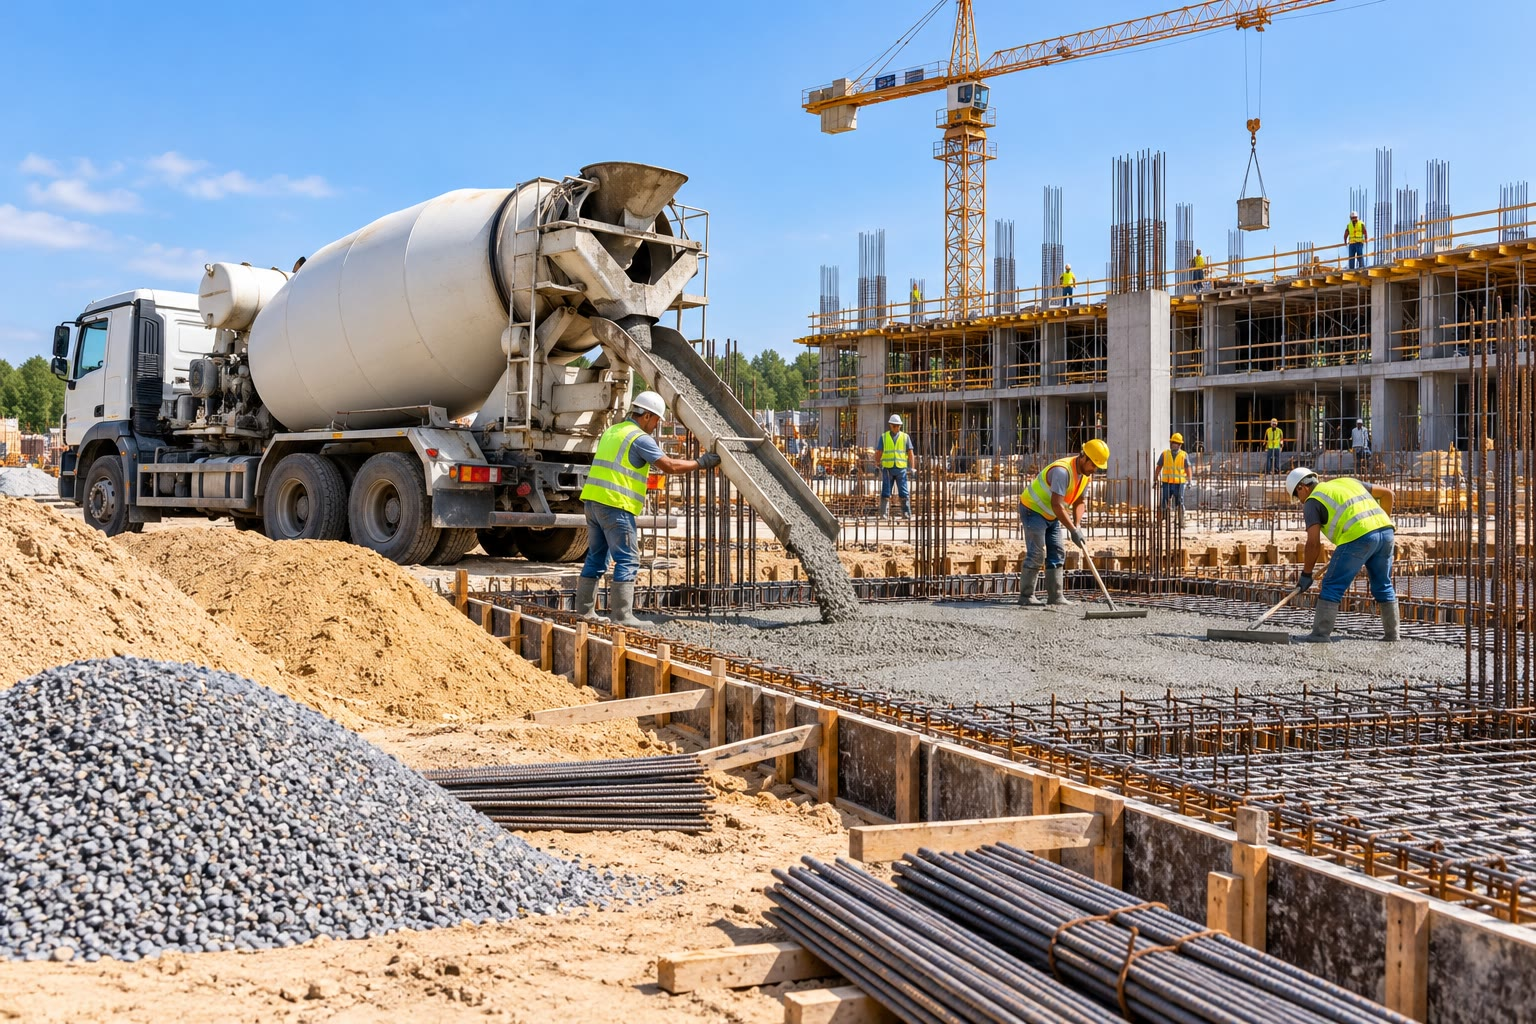
\includegraphics[width=\linewidth]{images/book1/ai/g9-building-site.jpg}
\end{minipage}\hfill
\begin{minipage}[c]{0.5\linewidth}\raggedright
{\small \omterm{def:g9:earth-resources:aggregate}{Aggregates} at work: heaps of \omterm{def:g3:stones-pebbles-sand:sand}{sand} and \omterm{def:g3:stones-pebbles-sand:pebble}{gravel} beside a concrete
mixer truck pouring the floor of a new building (AI-generated
illustration of a generic scene).}
\end{minipage}
\label{fig:g9:earth-resources:building-site}
\end{omfigure}

\section{Renewable or finite?}

A resource that nature renews within a human lifetime, like the water of
an \omterm{def:g6:water-underground:aquifer}{aquifer} that is not overpumped, can be used for ever. An \omterm{def:g9:earth-resources:ore-deposit}{ore deposit},
a coal seam or an oil field took millions of years to form. We use it in
a few decades: on our time scale, it is not renewed at all.
% ledger: eia:coal, earle:coal

\begin{omfigure}
\begin{tikzpicture}
\begin{axis}[xmode=log, width=12.5cm, height=4.6cm, xmin=10, xmax=1e9, ymin=0.4, ymax=4.6,
  ytick=\empty, xlabel={years (logarithmic scale)}, label style={font=\small},
  xtick={10,100,1000,1e4,1e5,1e6,1e7,1e8,1e9},
  xticklabels={$10$,$10^2$,$10^3$,$10^4$,$10^5$,$10^6$,$10^7$,$10^8$,$10^9$},
  tick label style={font=\footnotesize}, xmajorgrids, grid style={black!12}, clip=false]
\addplot[only marks, mark=|, mark size=4pt, line width=4pt, omWarm,
  error bars/.cd, x dir=plus, x explicit, error bar style={line width=4pt, omWarm}, error mark=none]
  table[x=lo_yr, y=y, x error expr=\thisrow{hi_yr}-\thisrow{lo_yr}] {figdata/out/grade-9-concentration-times.dat};
\node[anchor=west, font=\footnotesize, fill=white, inner sep=1pt] at (axis cs:1500,4) {a swamp builds a thick layer of plants};
\node[anchor=east, font=\footnotesize, fill=white, inner sep=1pt] at (axis cs:6e7,3) {age of coal mined in the United States};
\node[anchor=west, font=\footnotesize, fill=white, inner sep=1pt] at (axis cs:150,2) {Chuquicamata worked so far (over a century)};
\node[anchor=west, font=\footnotesize, fill=white, inner sep=1pt] at (axis cs:65,1) {world copper reserves at the 2024 mining rate};
\end{axis}
\end{tikzpicture}

{\small Times of making and times of using, on a scale where each step is
ten times the one before. The coal is about a million times older than
the time a mine takes to empty a deposit.}
% ledger: earle:coal, eia:coal, earle:chuquicamata, usgs:mcs-copper (figdata/grade-9/concentration.py, part times)
\label{fig:g9:earth-resources:times}
\end{omfigure}

How long will a resource last? Geologists count only what is known and can
be extracted.

\begin{definition}[Reserve]\label{def:g9:earth-resources:reserve}
The \emph{reserve}\index{reserve} of a \omterm{def:g6:rocks-and-minerals:mineral}{mineral} resource is the part of the
known deposits that can be extracted at a profit, with the techniques and
the prices of the day.
\end{definition}
% ledger: usgs:mcs-reserves

A \omterm{def:g9:earth-resources:reserve}{reserve} is not everything that is in the ground. It grows when new
deposits are found, when techniques improve or when prices rise, and it
shrinks as the deposits are mined. In 1970 the world's copper \omterm{def:g9:earth-resources:reserve}{reserves}
were estimated at 280~million tonnes. Since then, about 700~million tonnes
of copper have been mined, two and a half times that \omterm{def:g9:earth-resources:reserve}{reserve}, and yet the
\omterm{def:g9:earth-resources:reserve}{reserves} of 2024 were estimated at 980~million tonnes.
% ledger: usgs:mcs-reserves

\begin{dated}{2025}
In 2024 the mines of the world produced about 23~million tonnes of copper.
At that rate, the \omterm{def:g9:earth-resources:reserve}{reserves} of 980~million tonnes would last $980 \div 23
\approx 43$ years. Such a number is not a date when copper will run out:
it is a measure of the copper that is known and worth extracting today.
\end{dated}
% ledger: usgs:mcs-copper (figdata/grade-9/concentration.py: 42.6 years)

A metal, unlike coal or oil, is not destroyed when it is used: the
recycling of materials, met in the chemistry books, gives it back. The
copper of an old cable, of a scrapped engine or of the offcuts of a
factory can be melted and refined again. In the United States in 2024,
copper recovered from scrap made up about \qty{35}{\%} of all the copper
used.
% ledger: usgs:mcs-copper-scrap

\begin{omfigure}
\begin{tikzpicture}[font=\footnotesize, node distance=1.2cm,
  box/.style={draw=black!60, fill=black!4, rounded corners=2pt, align=center, minimum height=0.9cm, inner sep=3pt},
  flow/.style={-{Stealth[length=2.2mm]}, line width=0.9pt, black!70}]
  \node[box, fill=omWarm!12] (ore) at (0,0) {ore deposit\\(rock with \qty{0.5}{\%}\\of copper)};
  \node[box] (metal) at (4.2,0) {copper metal};
  \node[box] (things) at (8.2,0) {cables, pipes,\\engines};
  \node[box, fill=blue!8] (scrap) at (6.2,-2.1) {scrap};
  \node[box, fill=black!12] (waste) at (0,-2.1) {crushed rock\\left over};
  \draw[flow] (ore) -- node[above] {dig, crush,} node[below] {concentrate} (metal);
  \draw[flow] (metal) -- node[above] {make} (things);
  \draw[flow] (things) |- node[pos=0.25, right] {thrown away} (scrap);
  \draw[flow] (scrap) -| node[pos=0.75, left] {melt, refine} (metal);
  \draw[flow] (ore) -- (waste);
\end{tikzpicture}

{\small Two roads to copper metal: from an ore, through tonnes of \omterm{def:g3:stones-pebbles-sand:rock}{rock}
dug and crushed, or from scrap, which is melted and refined again.}
\end{omfigure}

\begin{example}[The rock that recycling saves]\label{ex:g9:earth-resources:recycling}
An ore with \qty{0.5}{\%} of copper holds \qty{5}{kg} of copper in each
tonne of \omterm{def:g3:stones-pebbles-sand:rock}{rock}. To make one tonne of copper, about $1000 \div 5 = 200$
tonnes of ore have to be dug, crushed and treated, and almost all of it
ends as waste \omterm{def:g3:stones-pebbles-sand:rock}{rock}. Each tonne of copper made from scrap leaves those 200
tonnes of \omterm{def:g3:stones-pebbles-sand:rock}{rock} in the ground --- and the deposit lasts longer.
% ledger: perkins:ore-grades (computed)
\end{example}


\section{Exercises}

\begin{exercise}[$\star$]\label{exo:g9:earth-resources:1}
Complete with the right word (\omterm{def:g9:earth-resources:ore-deposit}{ore deposit}, \omterm{def:g9:earth-resources:ore-deposit}{concentration factor}, \omterm{def:g9:earth-resources:aggregate}{aggregate},
\omterm{def:g9:earth-resources:reserve}{reserve}). (a) \omterm{def:g3:stones-pebbles-sand:sand}{Sand} used in concrete is an \ldots\ (b) The part of the known
copper that can be extracted at a profit today is the copper \ldots\ (c) A
\omterm{def:g3:stones-pebbles-sand:rock}{rock} where a metal is rich enough to be mined is an \ldots\ (d) The number
of times a metal has been concentrated is its \ldots
\end{exercise}

\begin{exercise}[$\star$]\label{exo:g9:earth-resources:2}
% ledger: earle:magmatic, usgs:gold-lode, usgs:gold-placer
Which way of concentrating a metal does each sentence describe: in the
\omterm{def:g7:volcanoes:magma}{magma}, in cracks from hot water, or in \omterm{def:g1:landscapes-around-us:water}{river} \omterm{def:g3:stones-pebbles-sand:pebble}{gravels}? (a) Gold nuggets lie
on the \omterm{def:g3:stones-pebbles-sand:rock}{bedrock} under a stream's \omterm{def:g3:stones-pebbles-sand:pebble}{gravel}. (b) Hot water fills a crack with
quartz and gold. (c) A layer of heavy nickel \omterm{def:g6:rocks-and-minerals:mineral}{minerals} lies at the bottom of
an old body of \omterm{def:g7:volcanoes:magma}{magma}. (d) Gold is freed from a vein by \omterm{def:g5:water-shapes-the-land:erosion}{erosion}.
\end{exercise}

\begin{exercise}[$\star$]\label{exo:g9:earth-resources:3}
% ledger: earle:coal, eia:coal
Put these steps in order: (a) the plant layer is buried under \omterm{def:g1:landscapes-around-us:water}{river} \omterm{def:g3:stones-pebbles-sand:sand}{sand};
(b) trees grow in a swamp; (c) a hard black coal forms kilometres down;
(d) dead plants pile up under still water; (e) a soft brown coal forms.
\end{exercise}

\begin{exercise}[$\star$]\label{exo:g9:earth-resources:4}
On the scale of a human life, is each resource renewable or not? Explain in
one sentence. (a) Coal. (b) The water of an \omterm{def:g6:water-underground:aquifer}{aquifer} pumped less than the
\omterm{def:g4:clouds-rain-snow:precipitation}{rain} refills it. (c) Copper ore. (d) The same \omterm{def:g6:water-underground:aquifer}{aquifer} pumped twice as fast
as it is refilled.
\end{exercise}

\begin{exercise}[$\star\star$]\label{exo:g9:earth-resources:5}
% ledger: perkins:ore-grades
Compute the \omterm{def:g9:earth-resources:ore-deposit}{concentration factor}, then write it as a power of ten, rounded:
(a) zinc, \qty{0.007}{\%} in the \omterm{def:g6:inside-the-earth:layers}{crust}, ore from \qty{4}{\%}; (b) tin,
\qty{0.0002}{\%} in the \omterm{def:g6:inside-the-earth:layers}{crust}, ore from \qty{0.5}{\%}; (c) iron,
\qty{5.6}{\%} in the \omterm{def:g6:inside-the-earth:layers}{crust}, ore from \qty{20}{\%}. (d) Why does iron need
so little concentration?
\end{exercise}

\begin{exercise}[$\star\star$]\label{exo:g9:earth-resources:6}
% ledger: usgs:gold-placer
Pure gold has a density of about \qty{19.3}{g/cm^3}; ordinary \omterm{def:g3:stones-pebbles-sand:rock}{rock} about
\qty{2.5}{g/cm^3}. (a) How many times denser is gold? (b) What is the mass
of a grain of gold of \qty{0.01}{cm^3}, and of a grain of \omterm{def:g3:stones-pebbles-sand:rock}{rock} of the same
size? (c) Explain why, in a \omterm{def:g5:water-shapes-the-land:flood}{flood}, the gold ends up at the bottom of the
\omterm{def:g3:stones-pebbles-sand:pebble}{gravel}, on the \omterm{def:g3:stones-pebbles-sand:rock}{bedrock}.
\end{exercise}

\begin{exercise}[$\star\star$]\label{exo:g9:earth-resources:7}
% ledger: perkins:ore-grades, earle:ore-grades (figdata/grade-9/concentration.py)
Use the chart of \omterm{def:g9:earth-resources:ore-deposit}{concentration factors}. (a) Which metals need a factor of
more than $10^3$? (b) Between which powers of ten does copper lie? (c) How
many times more does chromium need to be concentrated than aluminium?
(d) Which of the seven metals would you expect to find mined in the
fewest places? Explain.
\end{exercise}

\begin{exercise}[$\star\star$]\label{exo:g9:earth-resources:8}
% ledger: tos:sand
The world needs about \qty{18}{kg} of \omterm{def:g3:stones-pebbles-sand:sand}{sand} and \omterm{def:g3:stones-pebbles-sand:pebble}{gravel} per person and per
day. (a) How much is that per person in one year, in tonnes? (b) Write 50
billion tonnes in scientific notation. (c) A truck carries \qty{25}{t}.
How many days does it take for one person's share to fill it? (d) Why can taking \omterm{def:g3:stones-pebbles-sand:sand}{sand}
from a \omterm{def:g1:landscapes-around-us:water}{river} make a beach downstream shrink?
\end{exercise}

\begin{exercise}[$\star\star$]\label{exo:g9:earth-resources:9}
% ledger: earle:oil-gas, eia:oil
(a) From what living things do most oil and gas come? (b) Below about
\qty{2}{km}, at what temperatures does oil form? (c) Why do oil and gas
move upwards through the \omterm{def:g3:stones-pebbles-sand:rock}{rocks}? (d) What kind of \omterm{def:g3:stones-pebbles-sand:rock}{rock} stops them, and
where do they gather?
\end{exercise}

\begin{exercise}[$\star\star$]\label{exo:g9:earth-resources:10}
% ledger: earle:chuquicamata
The Chuquicamata mine has produced over 29~million tonnes of copper in
over 100 years. (a) Write 29~million tonnes in scientific notation. (b)
Roughly what is the average production per year? (c) If the ore held
\qty{1}{\%} of copper, how many tonnes of ore were dug to get 29~million
tonnes of copper? Use scientific notation. (d) Why does a mine of such a
poor ore have to be so large?
\end{exercise}

\begin{exercise}[$\star\star\star$]\label{exo:g9:earth-resources:11}
% ledger: usgs:mcs-reserves, usgs:mcs-copper
In 1970, the world's copper \omterm{def:g9:earth-resources:reserve}{reserves} were estimated at 280~million tonnes.
From 1970 to 2024, about 697~million tonnes were mined, and the \omterm{def:g9:earth-resources:reserve}{reserves}
of 2024 were 980~million tonnes, with 23~million tonnes mined in 2024.
(a) If the 1970 \omterm{def:g9:earth-resources:reserve}{reserve} had been all the copper there was, when would it
have run out? Compare with what was mined. (b) How many times larger is the
2024 \omterm{def:g9:earth-resources:reserve}{reserve} than the 1970 one? (c) Compute how many years the 2024
\omterm{def:g9:earth-resources:reserve}{reserve} would last at the 2024 rate. (d) Give two reasons why a \omterm{def:g9:earth-resources:reserve}{reserve} can
grow even while it is being mined.
\end{exercise}

\begin{exercise}[$\star\star\star$]\label{exo:g9:earth-resources:12}
% ledger: earle:coal, eia:coal
A coal seam is $3 \times 10^8$ years old. Its swamp lasted $2 \times 10^3$
years, and the seam is mined out in 50 years. (a) Write 50 years in
scientific notation. (b) How many times longer than the mining did the
swamp last? (c) How many times older than the time of mining is the seam?
(d) Use these numbers to explain why coal is called a non-renewable
resource.
\end{exercise}

\section{Problem: Concrete for a new town}

\begin{problem}[{Weekend problem --- a new town is built with the sand of a
local pit; the final answer is the number of years the pit's sand reserve
would last}]
\label{pb:g9:earth-resources:1}
% ledger: usgs:aggregate (about 100 and 300 t per home), tos:sand (figdata/grade-9/concentration.py, part problem: exercise data)
A new town of \num{2000} homes is to be built in ten years, near an old
\omterm{def:g3:stones-pebbles-sand:sand}{sand} pit dug in the \omterm{def:g3:stones-pebbles-sand:pebble}{gravels} of a \omterm{def:g1:landscapes-around-us:water}{river} terrace. Counting its share of the
streets, the schools and the shops, each home needs about \qty{300}{t} of
\omterm{def:g9:earth-resources:aggregate}{aggregates}, of which \qty{40}{\%} is \omterm{def:g3:stones-pebbles-sand:sand}{sand}. The pit's \omterm{def:g3:stones-pebbles-sand:sand}{sand} layer is
\qty{1.2}{km} long, \qty{500}{m} wide and \qty{5}{m} thick; one cubic metre
of its \omterm{def:g3:stones-pebbles-sand:sand}{sand} has a mass of \qty{1.6}{t}. The pit also sells
\num{136000} tonnes of \omterm{def:g3:stones-pebbles-sand:sand}{sand} a year to the rest of the region.

\noindent\textbf{Part I --- How much sand?}\par\nopagebreak
\begin{enumerate}[beginpenalty=10000]
  \item A family house alone needs about \qty{100}{t} of \omterm{def:g9:earth-resources:aggregate}{aggregates}. Write
        this mass in kilograms, in scientific notation.
  \item How many tonnes of \omterm{def:g9:earth-resources:aggregate}{aggregates} will the whole town need?
  \item How many tonnes is that per year, over the ten years?
  \item How many tonnes of \omterm{def:g3:stones-pebbles-sand:sand}{sand} per year does the town need?
\end{enumerate}

\noindent\textbf{Part II --- The reserve.}\par\nopagebreak
\begin{enumerate}[resume, beginpenalty=10000]
  \item Compute the volume of the \omterm{def:g3:stones-pebbles-sand:sand}{sand} layer, in cubic metres, in
        scientific notation.
  \item A third of the layer lies under a village and a road and will
        not be dug. What volume can be extracted?
  \item What is the mass of this \omterm{def:g9:earth-resources:reserve}{reserve}, in tonnes?
  \item How many tonnes of \omterm{def:g3:stones-pebbles-sand:sand}{sand} will the pit sell each year, to the town
        and to the region together?
\end{enumerate}

\noindent\textbf{Part III --- Renewable or not?}\par\nopagebreak
\begin{enumerate}[resume, beginpenalty=10000]
  \item Each year, the \omterm{def:g1:landscapes-around-us:water}{river} brings about \num{2000} tonnes of new \omterm{def:g3:stones-pebbles-sand:sand}{sand} to
        the area. How many times more \omterm{def:g3:stones-pebbles-sand:sand}{sand} does the pit sell?
  \item On the scale of the town's life, is this \omterm{def:g3:stones-pebbles-sand:sand}{sand} a renewable
        resource? Explain.
  \item If the town replaced a quarter of its \omterm{def:g3:stones-pebbles-sand:sand}{sand} with crushed old
        concrete, how many tonnes of \omterm{def:g3:stones-pebbles-sand:sand}{sand} would it save each year?
  \item Without that recycling, how many years would the pit's \omterm{def:g3:stones-pebbles-sand:sand}{sand}
        \omterm{def:g9:earth-resources:reserve}{reserve} last?
\end{enumerate}
\end{problem}
